\documentclass[12pt]{article}


\usepackage{amsfonts}
\usepackage[parfill]{parskip}
\usepackage{caption}
\usepackage{enumerate} 
\usepackage[pdftex]{graphicx}
\usepackage[top=2cm, bottom=2cm, left=2cm, right=2cm]
{geometry}
%\usepackage[rightcaption]{sidecap}
\usepackage{subfig}
\usepackage [english]{babel}
\usepackage{natbib}
\usepackage [autostyle, english = american]{csquotes}
\usepackage{setspace}
\MakeOuterQuote{"}
\graphicspath{{./plots/}}
\captionsetup[table]{skip=12pt}
\bibliographystyle{plainnat}


\begin{document}







% ======================================================================================================
% Title page
% ======================================================================================================


\title{The quantification of DNA motifs within flanking sequences of gene expression quantitative trait loci in humans: Laboratory Report}

% Authors
% ----------

\author{Jacqueline Kiewa}





\doublespacing
\maketitle
\clearpage
\tableofcontents
%--------------------------------------------------------------------------------------------------------------------------%
%--------------------------------------- Begin Document -----------------------------------------------------------%


%--------------------------------------------------------------------------------------------------------------------------%
%--------------------------------------- Introduction-------------------------------------------------------------------%
\clearpage
\section{Introduction}

An important complex trait that differs amongst individuals is the level of gene expression, obtained by measuring the amount of mRNA present in specific tissues. The class of variants that influence this trait has been labelled expression quantitative trait loci (eQTL). These variants are particularly important to Genome Wide Association (GWA) studies, since they can help to prioritize likely causal variants amongst the SNPs identified by the GWA study, as well as provide some insight into the biological mechanisms used by organisms to influence complex traits and diseases \citep{albert2015role}. \citet{albert2015role} note that the majority of QTL identified by human GWA studies occur in non-coding regions that are not in linkage disequilibrium (LD) with coding exons. It is therefore hypothesised that these QTL influence their targeted gene through regulation of its expression \citep{nica2013expression}. A further hypothesis is that an eQTL and its surrounding region will be enriched in biologically active DNA sequence motifs which will contribute in some way to gene expression regulation. 

\citet{lloyd2017genetic} conducted an analysis using data from the Consortium for the Architecture of Gene Expression (CAGE), which comprises individual-level whole-blood expression and genotype data on 2,765 individuals. This analysis identified a total of 14,995 expression quantitative trait loci (eQTL), of which 11,204  were in cis. The aim of this research is to identify DNA motifs in the genomic regions surrounding the set of cis eQTL identified by \citet{lloyd2017genetic}, following the hypothesis that flanking sequences of an eQTL will be enriched in recurring motifs of DNA that have a biological function, most likely involved in transcription.

\subsection{Motif function}
DNA sequence motifs are short, recurring sequences in DNA that are thought to have some biological function \citep{d2006dna}. They may form binding sites for proteins such as transcription factors or nucleases, or they may provide signals for important regulatory processes such as methylation, or ribosome binding or mRNA processing \citep{d2006dna}. Gene regulation is an important aspect of the eukaryotic genotype \citep{beckerman2005gene}, changes in which are responsible for much of the phenotypic divergence between and within species \citep{stewart2012transcription}. However, an understanding of the biological mechanisms by which this diversity regulates gene expression has been challenging  \citep{pai2015genetic, gaffney2013global}. Transcription constitutes the first and one of the most intensely regulated steps of gene expression \citep{zabidi2016regulatory}, and a subset of DNA motifs in the region of eQTL are sequence binding sites for transcription factors (TFs). Much research has therefore focused on the identification of transcription factors that coincide with eQTL and are likely to enhance or restrict gene expression. 


Once chromatin has become accessible, transcription can initiate within the core promoter site, which recruits RNA polymerase II and assembles the pre-initiation complex \citep{zabidi2016regulatory}. However, transcription will proceed at a very low basal level without the contribution of enhancers. Enhancers are DNA elements up to several hundred bp in length, and contain many short TF binding sites. Either individual or cooperative combinations of TFs are recruited to these sites and function as activators or repressors that regulate transcription from the target core promoter. Despite the abundance of research that has focussed on the relationship between eQTL and transcription factors, as a subset of DNA sequence motifs, TFs form just one piece in the complex jigsaw of gene regulation, with other regulatory processes also playing a part. A de novo motif search by \citet{schor2017promoter}, for example, found a number of core motifs (not TF binding sites) that controlled the shape of promoter regions, resulting in changed transcription levels. Other systems of gene regulation include methylation of CpG sites, alternative splicing, and post-transcriptional effects such as interaction with miRNAs and polyadenylation \citep{gaffney2013global}. \citet{gaffney2013global} also observed that eQTL are often enriched in exons, and \citet{kirsten2015dissecting} found that eQTL also coincide with non-coding RNAs and pseudogenes.
 
The following overview of potentially important motifs in DNA follows that of \citet{boeva2016analysis}. 

Tandem repeats are repeated DNA sequence ordered in a head-to-tail fashion and include microsatellites, minisatellites, and satellite sequences. Short tandem repeats (STRs) may serve as binding sites for specific transcription factors, whilst longer satellite repeats can influence the 3D structure shaping of the genome. Interspersed repeats are similar sequences to STRs and are located throughout the genome and include transposable elements such as SINEs and LINEs. 

AT-rich sequence are often located in gene promoters and play a role in transcription initiation. Approximately 24\% of human genes contain an AT-rich sequence within the core promoter, with 10\% containing a canonical TATA-box motif (TATAWAWR; W = A/T, R = A/G). In general, AT-rich DNA is easier to unwind than GC-rich DNA, since AT base pairing contains fewer bonds than GC base pairs, but this process is amplified by TATA binding protein which is recruited by the TATA-box. 

The remaining 76\% of human promoters that are GC-rich contain multiple binding sites of the transcriptional activator SP1 \citep{yang2007prevalence}. As much as 56\% of human genes, including most housekeeping genes, possess CpG islands, i.e. 300-3000 bp GC-rich sequences around gene transcription start sites (TSS's) with a high density of CpG dinucleotides. CpG islands have a high methylation level, which is associated with transcriptional repression. 

Splice sites are involved post initial transcription, when the RNA undergoes the process of splicing, during which introns are removed and the remaining exons are joined together. Generally this process is catalyzed by spliceosomes that recognize a donor site, which is almost invariably `GU' at the 5' end of the intron; a branch site, which is an `A' followed by a pyrimidine-rich tract near the 3' end of the intron; and an acceptor site, which is almost always `AG' at the 3' end of the intron. A DNA mutation in a splice site may have a wide range of functional consequences often leading to a defective or truncated protein.  

Micro RNA molecules (miRNA's) regulate the amount of protein at the post-transcriptional level. Micro RNA's form part of the RNA-Induced Silencing Complex (RISC). The function of miRNA in this complex is to bind to the 3' untranslated region of of messenger RNA (mRNA). A successful binding will lead to repression of the translation of mRNA into protein. Mutations in an miRNA target site can therefore disrupt miRNA repressive regulation, resulting in protein over expression.

\subsection{Motif detection}
DNA motif detection can be done experimentally or with high-throughput data analysis using computer algorithms. Identification of DNA motifs can be achieved through in vivo or in vitro experiments, which include, for example, ChIP-seq (in vivo) that uses actual TF binding events in particular biological conditions, such as cell type or treatment time point \citep{inukai2017transcription}. In vitro approaches (e.g. SELEX) use artificially created DNA and are well suited for large-scale characterization of intrinsic TF binding sequence preferences \citep{inukai2017transcription}.  Results from a ChIP-seq experiment typically have a resolution of approximately 100 bp, and the set of sequences identified as a result of the experiment (ChIP-seq data) becomes the focus of a search for a single motif of the particular transcription factor used within the binding experiment, i.e. one motif that is the best match over all sequences identified within the experimental process. This process has been termed `OOPS', or one occurrence per sequence \citep{zhang2016entropy}. This consensus motif is putatively labelled as a TFBS for the bound transcription factor identified within the experimental data. 

Alternatively, computational based motif detection searches for short lengths of DNA that have been conserved across sequences, but is not limited to one motif per sequence or to transcription factor binding sites (TFBS's). Zero, one, or multiple different motifs per sequence can be identified. The conservation of these motifs is thought to indicate biological significance. This significance is not necessarily that of a TFBS, but might be due to some other factor, as described in section 1.1 above. 

As for single motif finding tools, multiple motif finding tools were first developed for finding transcription factors \citep{dassi2016dynamit}, and many of them require ChIP-seq sequences as input. Later tools were developed to find other motifs, but again often focused on a particular section of DNA, such as promoters or enhancers  \citep{boeva2016analysis}.

\citet{das2007survey} describe motif discovery as one of the most challenging problems in molecular biology and computer science, and formulate it as follows:
given a set of sequences, find an unknown pattern that occurs frequently. If a pattern of $m$ letters long appears exactly in every sequence, a simple enumeration of all $m$-letter patterns that appear in the sequences gives the solution. To find this pattern, in a set of $t$ sequences of length $n$, we need to consider all $(n - m +1)t$ possible starting positions or candidates for motifs. 

The problem increases in complexity with the introduction of $d$, which is the number of point changes that will be accepted in any motif instance. This change might take the form of a simple change in nucleotide (e.g. from an A to a T) or of an insertion or a deletion. Since an exact match may not exist, the motif detection algorithm must consider all possible combinations of ``words" of the given length across all sequences. Thus the problem becomes exponential with the number of sequences. For each combination, the detection algorithm must perform an alignment and calculate the probability that this combination of ``words" are instances of the same motif. At the end of this process, the combination of ``words" with the best probability will become the basis for a Position Weight Matrix which will be the accepted consensual motif for this group of sequences. 

Given this level of complexity, the motif finding problem is an example of an NP-complete problem \citep{tran2014survey} (NP $:$ nondeterministic polynomial time). A solution to the search problem can theoretically be found and verified in polynomial time by a nondeterministic algorithm which has the power of guessing correctly at every step \citep{dasgupta2006algorithms}. However, although such an algorithm theoretically exists, no polynomial time algorithm has yet been discovered for an NP-complete algorithm \citep{cormen2009introduction}.  Algorithms for solving this problem can be categorised as per \citep{sun2015affinity}, who grouped algorithms into exact algorithms, which achieve efficiency through organisational pre-processing such as a suffix tree to reduce the search space; and approximate algorithms, which use heuristic methods such as expectation maximisation to reduce processing time.

\subsection{Conceptual example of a motif detection algorithm, and the Position Weight Matrix}
This section will be used to describe one motif finding algorithm: the Gibbs algorithm \citep{Lawrence1993Gibbs}. A conceptual example will be provided, following the teaching videos provided by \citep{Algoshareify}.

The example begins with a set of sequences, $n=10$ and $t=4$, in which we are to find one example of a motif $M$ of length $l=7$ in each sequence:
\begin{center}
A  C  C  A  T  G  A  C  A  G\\
G  A  T  T  A  T  A  C  C  T\\
C  A  T  G  C  T  T  A  C  T\\
C  G  G  A  A  T  G  C  A  T\\
\end{center}
The algorithm works through repeated iterations of a single process. Each iteration ends with a choice of starting position for the motif in one of the sequences.

An iteration begins by setting one sequence aside as the target sequence. This sequence is chosen randomly, but in this example (see Figure \ref{gibbs1}, the first sequence (marked in red) will be used as the random sequence . All other sequences form the background. The background sequences are used to create a frequency table, which is then used to calculate the probability of the motif occurring at each possible position in the target sequence.

To construct the frequency table, first a motif position is chosen, at random, for each background sequence. In Figure \ref{gibbs1} the background motifs are marked blue. Next the blue elements in the table are filled in according to the counts of the nucleotides for each position in the background motifs. The column headers in the table indicate the positions in the motifs. The green column (with the zero header) is filled in according to the counts of nucleotides in the non-motif background, irrespective of position. This creates the following scenario:

\begin{figure}[!htbp]
\centering
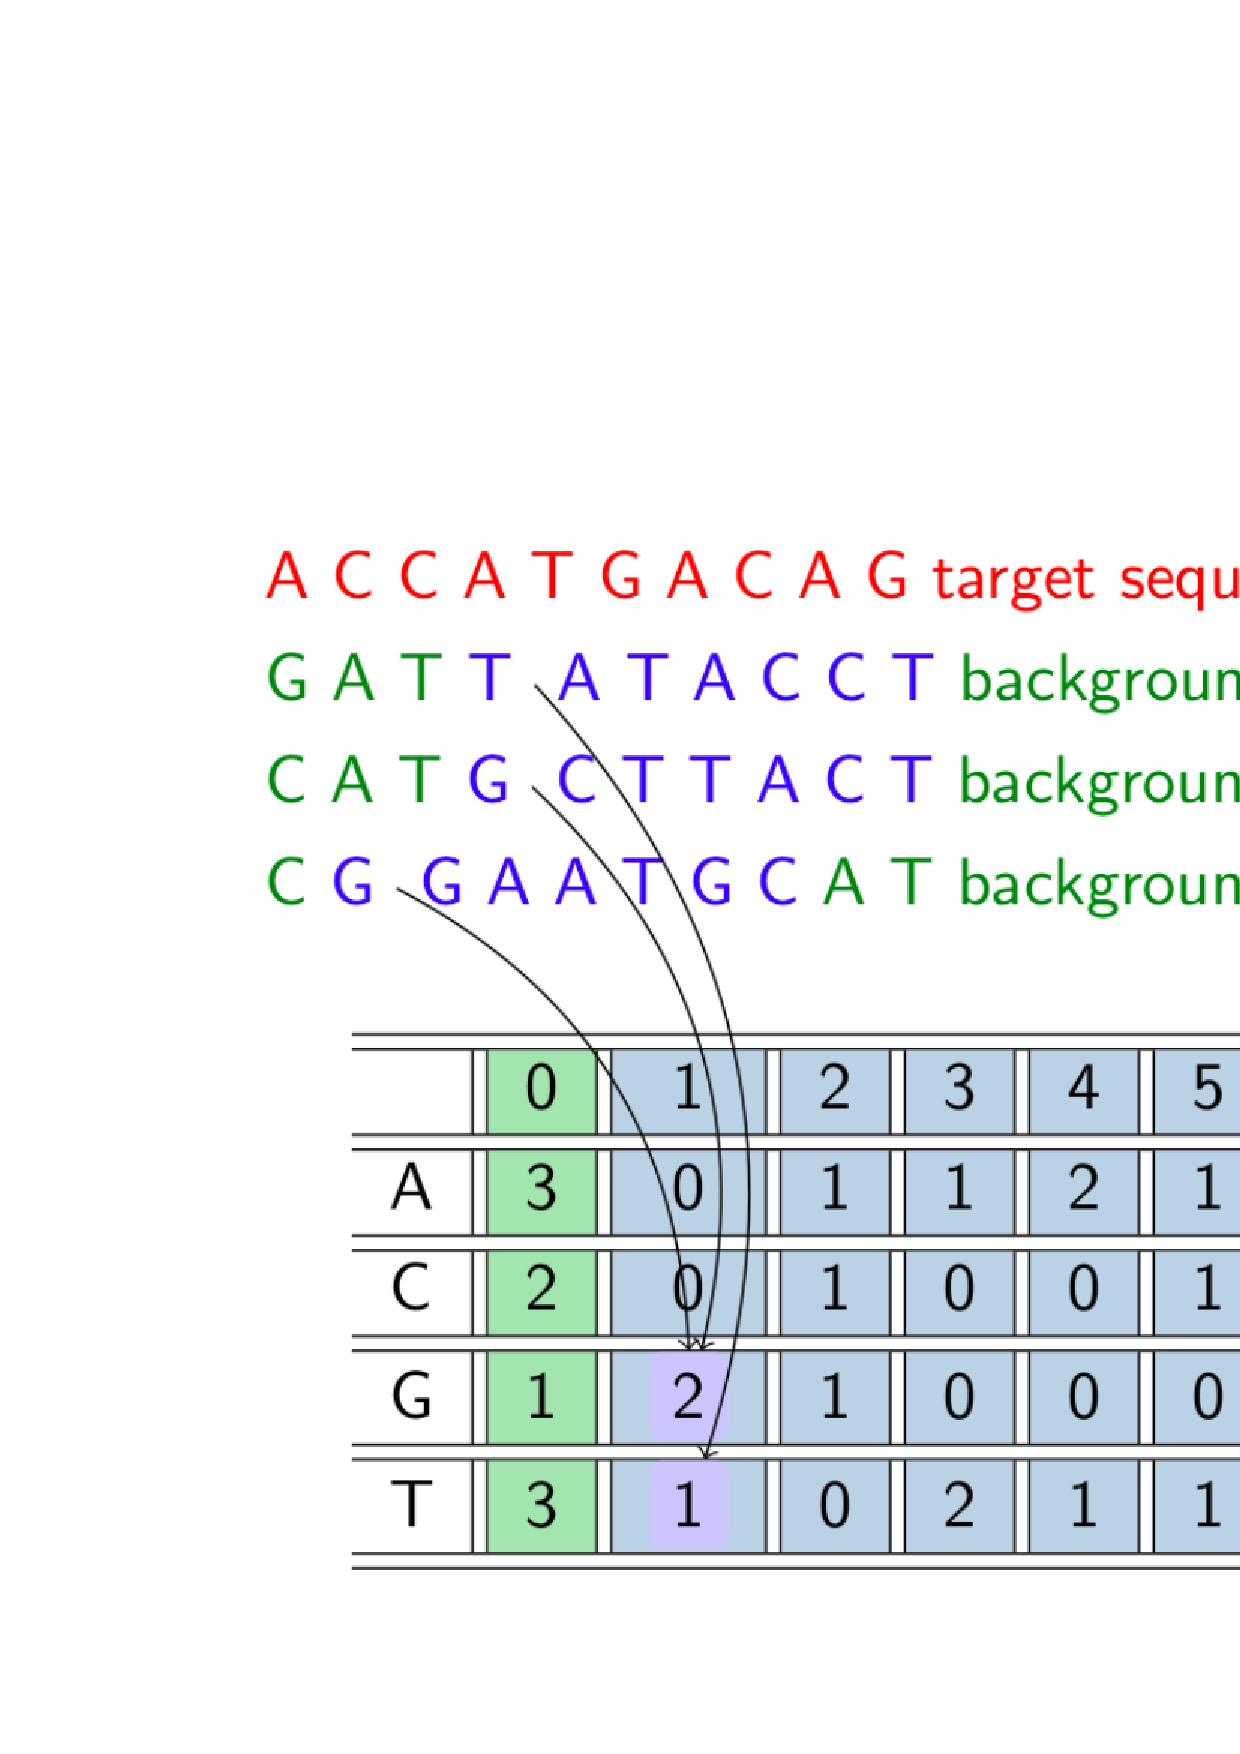
\includegraphics[width=0.7\textwidth]{GibbsTable.png}
\caption{Gibbs algorithm: creating the frequency table}\label{gibbs1}
\end{figure}

Pseudocounts are added to the counts in the table to eliminate zero's, and counts are turned into frequencies by dividing by the number of sequences (for the blue columns) or the total number of non-motif nucleotides (for the green column).

The second part of the iteration returns to the target sequence. For each possible motif starting position in this sequence, the probability of the resultant motif is worked out using the frequency table and the following equation: 
\begin{equation}
p(M_{1}) = \frac{p_{1,A} \cdot p_{2,C} \cdot p_{3,C} \cdot p_{4,A} \cdot p_{5,T} \cdot p_{6,G} \cdot p_{7,A}}{p_{A} \cdot p_{C} \cdot p_{C} \cdot p_{A} \cdot p_{T} \cdot p_{G} \cdot p_{A}}
\end{equation}
This procedure is illustrated in Figure \ref{gibbs2}. As illustrated in this figure, each element in the numerator is found by referincing the corresponding motif position (column) and nucleotide (row) in the table. Each element in the denominator is found by referencing the corresponding nucleotide in the zero column, irrespective of position. The lower table displays the values calculated for each of the four possible motif starting positions.  

\begin{figure}[!htbp]
\centering
\includegraphics[width=0.7\textwidth]{GibbsTable1.png}
\caption{Gibbs algorithm: calculating the probability of the first motif start position}\label{gibbs2}
\end{figure}

The lower table of motif probabilities is normalised, and then used to weight a random choice of motif start position for the target sequence. This choice of motif for the target sequence is the culmination of this iteration. After hundreds of such iterations, depending on the number of sequences, motif positions will no longer be totally random, but most will have been weighted according to the procedure described above. After a certain number of iterations, a log likelihood of the probability of the current set of motifs is taken. If this log likelihood is better than the previous, it is retained; otherwise it is discarded and the algorithm returns to the motif positions for the previous log likelihood.

After many thousands of iterations the log likelihood is never better than the previous, and the algorithm will always return to the previous log likelihood. At this point convergence has been reached and a position weight matrix can be calculated for the set of motifs found.

The position weight matrix (PWM) itself is a useful tool that ensures that no information is lost with respect to the consensual motif sequence, since it records the frequency of each nucleotide in each position over all sequences (the position frequency matrix) before working out the probabilities for the final PWM. Another advantage is its convenient visualisation as a sequence logo, and a number of data bases (e.g. JASPAR \citep{Mathelier2016}; Hocomoco \citep{Kulakovskiy2018} and UniPROBE \citep{Hume2015}) now store many hundreds of PWMs that match every known transcription factor. In fact the PWM \textit{is} the motif, rather than the consensual sequence. The main disadvantage of the PWM is its assumption of independence of each position within the binding site, which may not always be true \citep{Jayaram2016}. However, as \citet{Jayaram2016} points out, in practice, PWM models tend to perform as well as more complex models that attempt to include nucleotide interdependencies in their calculations, but which are often more prone to learning noise.

\section{The Pilot Study}
\subsection{Introduction to the Pilot Study}
Computationally efficient algorithms were required for this analysis and thus a possible set of highly-used algorithms were evaluated via a pilot study using a set of 201 base pair regions with the full set of 14,995 cis and trans eQTLs, which reduced to 13,930 eQTLs once duplicates were removed. The results from the pilot study were used to guide a larger investigation into the the frequencies of detected motifs across the cis sequences, and the identification of transcription factors with binding sites that match the final list of motifs and characterise the biological function of detected motifs. These analyses will give insight into the regulation of gene expression in regions of the genome that contribute to variation of gene expression in whole blood. 

The general hypothesis is that if DNA motifs are detected in these sequences then we would expect them to have a common regulatory process across a subset of genes that harbour eQTL in the nearby region. This becomes a search for a conserved set of mechanisms across blood gene expression that acts through DNA motifs. This project sought to establish first whether it is indeed the case that DNA motifs can be detected in a robust manner.




\subsection{Organisation of the data}

The purpose of the pilot study was to investigate the possible methods for the identification of motifs associated with eQTLs identified by  \citet{lloyd2017genetic}. Short target sequences of 201 base pairs, centred on the full set of each independent eQTL (both cis and trans) from the CAGE analysis, formed a set of 13,930 sequences for the pilot investigation. These sequences were constructed using the Genome Reference Consortium Human Build 37 (GRCh37)\citep{Lander2001}, also known as hg19. Using the UCSC Table Browser \citep{karolchik2004ucsc} as a reference, these sequences were then divided into four subsets according to their location in the genome: exons; introns; promoters; and intergenic. This division into smaller subsets reduced running time within each class. Table \ref{freqComparisons} provides the number of target sequences that overlapped with these classes. Where a sequence overlapped with more than one class, it was included in both groups; hence the figures add up to more than the 13,930 sequences.

Discriminative algorithms search for motifs that are overrepresented in target sequences compared to background sequences. Since such motifs may account for the increased expression of genes associated with the target eQTLs, a discriminative approach seems ideally suited to this project.It became necessary, therefore, to identify a background set of sequences. For this set, sequences were centred on a random group of 17,226 variants from the CAGE study that have no effect on gene expression. Sequences associated with these variants (null sequences) were also divided into exon, intron, promoter and intergenic subclasses. The number of null sequences in each class is also provided in Table \ref{freqComparisons}. 

\begin{table}[!htbp]
\centering
\caption{Comparison of target and background sequences across classes}\label{freqComparisons}
\begin{tabular}{r|cccc|c}
\hline
Class & Exon & Intron & Promoter & Intergenic & Totals\\ \hline
Target Sequences & 2131 & 7834 & 1231 & 5132 & 16328\\ \hline
Background Sequences & 387 & 6886 & 256 & 10202 & 17731\\ \hline
Totals & 2518 & 14720 & 1487 & 15334 & 34059
\end{tabular}
\end{table} 

A comparison of the target and background sequence frequencies (see Table \ref{freqComparisons}) found significant differences in the numbers for each class across target and background sequences ($\chi^2$ = 3532.8, $p <$ 0.00001). Comparatively few of the null variants fell into exon or promoter sequences, but almost twice as many null variants compared to eQTLs fell into intergenic sequences. There was little difference between nulls and eQTLs with respect to the likelihood that they might be within an intron sequence.


 
\subsection{Potential motif algorithm set}

An initial literature review provided some insight into the types of algorithms that can be used to identify motifs. The OMICTools directory \citep{henry2014omictools} was used to provide a list of motif-finding algorithms. The following criteria was used as a guide to the choice of motifs:
\begin{itemize}
\item Used a discriminative algorithm (comparing frequency of motif in target sequences compared to background sequences);
\item Number of citations;
\item Represented different approaches to the Planted Motif Problem;
\item Ease of use (some programs were very difficult to install, or were no longer maintained and wouldn't run at all); and
\item Appropriate for eQTL sequences: Some algorithms are written for specific sequence sets, such as promoters, and it is unclear whether they are generally applicable to other types of sequences. Where possible algorithms that are specifically described as broadly applicable were used.
\end{itemize}

Based on these criteria, six algorithms: DREME, HOMER, motifRG, STEME, BaMM!motif and DECOD were eventually chosen for comparison. A brief overview of each motif follows.


DREME (Discriminative Regular Expression Motif Elicitation) \citep{bailey2011dreme} uses an enumerative algorithm, which is exact in the sense that it examines each possible 'word' in the sequence, which is very inefficient, with time increasing exponentially with the size of the motif and the number of sequences. DREME achieves efficiency by limiting the size of the motifs found, as well as a few shortcuts. Exact enumeration is used for seed motifs restricted to 3-8 base pairs in length, and significance established through comparison with the background sequence, using Fisher's Exact Test. The motif with the highest significance is used to create a set of non-overlapping occurrences in the set of sequences that are aligned to create a position-specific probability matrix. Following this step, the motif is `erased' and the search repeated.
 
HOMER \citep{heinz2010simple} begins by weighting background sequences to resemble the same GC-content distribution of the target sequences, since enrichment scores used in the motif detection algorithms might fail if the distribution of the length of GC content of the target sequences significantly
differs from the background set. Input sequences are then ``parsed" to gather all oligos of the desired motif length and read into an oligo table that records how many times each oligo occurs in the target and background sequences. These frequencies are used to calculate the relative enrichment of each oligo, using cumulative binomial distribution. The enrichment of longer oligos are calculated using the enrichment values of smaller oligos that make up the longer oligos, similar to the DREME method of combining seed significances. The most enriched oligos are then subjected to a local optimization algorithm which uses a probability matrix to score each oligo according to its similarity to the matrix. By decreasing the detection threshold, more oligos can be included, until an optimal enrichment is found. New probability matrices can then be created at different detection levels, and the matrix that results in the highest enrichment will be used to produce the final motif. This motif is then masked from the sequences and the whole process repeated to find the next motif \citep{homer_ws}.

MotifRG \citep{yao2014discriminative} begins by counting all $k$-mers, for a given motif length $k$, in all sequences. The motifRG algorithm uses logistic regression to fit a model with the best absolute z-value (which needs to be above an enrichment threshold). The chosen $k$-mer is used as a seed motif, which is then refined by stepped extension of a given number of nucleotides on each end of the seed at a time. Refinement ends when no further improvement in the z-score results after two successive steps. Small perturbations in the seed motif are then tried and accepted if the z-score is thereby improved, followed by the extension process. Since a small difference in the z-value may not be meaningful, a simple bootstrap test is done if the difference falls below a threshold. A default of 5 random samples of the sequences are used to calculate z-values for the new and original motifs. These z-values are then subjected to a t-test to establish whether their difference is significant.
Once the motif is established, it is masked from all sequences and the process begun again.

STEME (Suffix Tree EM for Motif Elicitation) \citep{reid2011steme} is modelled on the well established MEME algorithm \citep{bailey2009meme}, which uses Expectation Maximisation (EM), and this short review begins with a brief description of this process. EM is an extremely robust algorithm but each iteration begins with a time-inefficient initialisation step that generates a matrix of each possible motif and fills in the probability of each base by counting the number of times each base occurs in each position in the set of all motifs and dividing by the number of times it could have occurred (= the number of motifs). The expectation step uses the matrix to calculate the probability of each motif, and then this probability is used to weight the count of bases in the matrix (the maximisation step). The expectation and maximisation (E and M) steps are repeated until convergence is reached and the matrix no longer changes. The EM algorithm is subject to local optimas, and the solution adopted by MEME, to rerun the algorithm with different initial starting positions, results in a running time that is quadratic to the number of sequences and is not practicable with large data sets. STEME modifies the EM algorithm by ignoring all W-mers (subsequences of length W) which have a probability less than some threshold. In addition, STEME uses a suffix tree to iterate over all W-mers. Once the initial matrix is built, it is the content rather than the position of the W-mer that is relevant. A suffix tree can then achieve efficiency over the EM algorithm in two ways: firstly, if any two W-mers are identical they do not have to be repeated; and secondly, partial evaluations are calculated for each step of the suffix tree and shared across W-mers below that node in the tree. In contrast, MEME evaluates every base in each W-mer individually. STEME was still the slowest of these algorithms to run, but its authors claim that it is one order faster than the MEME algorithm with the same data \citep{reid2011steme}.

BaMM!motif (Bayesian Markov model or BaMM) \citep{siebert2016bayesian} addresses the issue that position weight matrices (PWMs) assume independence of each base in the motifs \citep{Jayaram2016}, which may not always be true. By using a Markov Model, the BaMM algorithm incorporates the probability of prior nucleotides into the final probability of any nucleotide in a particular position. BaMm begins with a 5th order Markov Model and uses expectation maximisation to estimate the transition and emission probabilities of these potential motifs. Probable motifs are lengthened using a Bayesian approach of multiplying the probability of the preceding markov model with the probability of the proposed additional nucleotide. Because the tables of probabilities produced by this algorithm have incorporated a higher order Markov modelling, the authors refer to them as BaMMs rather than as PWMs, although their layout is the same \citep{siebert2016bayesian}.

DECOD (DECOnvolved Discriminative motif finder) \citep{huggins2011decod} begins with an enumeration step: given a user-specified motif length $k$, all $k$-mers are extracted from the target and background sequences and arranged into a table of frequencies of occurrence. However, after this step, no further analysis is conducted of the actual sequences - all subsequent analysis is of the $k$-mer counts table and PWMs are formed on the basis of frequency of occurrence in target compared to background sequences. This heuristic approach greatly speeds up the algorithm but bears the cost of losing the context of the $k$-mer. This loss of context may mean that overlapping $k$-mers are counted for the same motif more than once, leading to a convolved PWM that is inaccurate. To overcome this problem DECOD adopts a deconvolution process that removes $k$-mers that form a subset of the true motif  \citep{huggins2011decod}.

Using six motif-finding algorithms with four classes of sequences meant that many motifs were produced. Manual comparison of motifs across algorithms searching for similarities amongst results became very difficult. 

The STAMP algorithm \citep{mahony2007stamp} was designed for this purpose. It has two main functions:
1. To perform motif alignment and group motifs according to similarity; and
2. To search the user's database of choice for known transcription factors with similar motifs.  STAMP provides a large number of user options:

\begin{enumerate}
\item Alignment of motifs can be according to Needleman-Wunsch (global) or Smith-Waterman (local) alignment methods;
\item These methods are based on column comparison scores calculated by one of five distance metrics: Pearson's correlation coefficient; Kullback-Leibler information content; sum of squared distances; average log-likelihood ratio; or average log-likelihood with a lower limit of -2.
\item Alignment can be gapped or ungapped with a variety of penalties imposed for gap-opening and gap-extension;
\item Users may choose to trim edges of motifs;
\item Motif multiple alignment strategies can be according to `progressive profile alignment' or `iterative refinement';
\item  Two tree building algorithms are offered: an agglomerative method (UPGMA) and a divisive method based on a self-organising tree algorithm (SOTA);
\item Five databases are offered for motif matching.
\end{enumerate}
\subsection{Results of the pilot study}

A disparate number of motifs were detected for each algorithm, which was a source of confusion. Table \ref{motif_summary} outlines some of the source of this confusion.

\begin{table}
\centering
\caption{Summary of motif detection algorithm properties.}\label{motif_summary}
\begin{tabular}{| p{2cm} |  p{2cm} |  p{2cm} |  p{6cm} |}
\hline
\textbf{Algorithm} & \textbf{No. of motifs option} & \textbf{Entered} & \textbf{Result}\\
\hline
DREME & Required & 15 & Stops finding motifs once a minimum threshold is reached\\
\hline
HOMER & Optional & Used a default of 25 & Finds 25 motifs for every length motif requested. Since 3 lengths were default, 75 motifs were returned\\
\hline
STEME & Required & 20 & Always finds the requested number of motifs, but often reports e-values above any useful threshold\\
\hline
DECOD & Required & 20 & Often does not find requested number of motifs, but no information supplied in the documentation to explain any thresholds\\
\hline
BaMM & No options & No default & No information provided re thresholds. Varying numbers of motifs resulted, but always with useful e-values\\
\hline
MotifRG & Optional & 20	& Has threshold minimum fraction of target/background sequences (=0.01) and minimum fold change of motif in target Vs background (=1.3)\\
\hline

\end{tabular}
\end{table}


The algorithms also varied in the statistical details provided to support their findings, as described in Table \ref{statisticaldetails}.

\begin{table}[!ht]
\centering
\caption{Comparison of provision of statistical details across algorithms}\label{statisticaldetails}
\begin{tabular}{| p{0.1\linewidth} |  p{0.2\linewidth} |  p{0.2\linewidth} |  p{0.4\linewidth} |}
\hline
Algorithm & Enrichment & p-value/E Value & Other details\\
& Calculation & provided &\\ 
\hline
DREME & Fishers Exact Test & Provides p-values and associated e-values &\\
\hline
HOMER & Cumulative binomial distribution & Provides uncorrected p-values & Provides the number of target and background sequences that contain the motif\\
\hline
STEME & Not provided & Provides e-values & Provides target and background numbers within mass of log data (difficult to locate)\\
\hline
DECOD & z scores & Provides e-values & E-values only provided for the GUI-version, not for the terminal command\\
\hline
BaMM & Log-odds score & Provides e-values & Varying numbers of motifs produced with significant e-values. Documentation states that threshold is $p<1.0$, but this is not reflected in results, which have very small E Values.\\
\hline
motifRF & Wald test & Not provided &\\
\hline


\end{tabular}
\end{table} 


Running the algorithms on each subset of the data resulted in a set of motifs for each sequence subset. Within each subset, motifs were formatted as input for the STAMP algorithm, which performed motif alignment across all motif sets and grouped the motifs according to similarity. Default parameters were used: Pearson Correlation Coefficient for distance metrics; Smith-Waterman local alignment ungapped alignment: Iterative refinement multiple alignment; UPGMA tree building; and the JASPAR database \citep{sandelin2004jaspar} to identify those motifs that corresponded to a known transcription factor.  

No strong differences emerged in the results from the four groups (exon, intron, promoter, and intergenic). Since the purpose of the pilot study was to evaluate the algorithms, rather than to do an indepth study of motifs found and associated transcription factors, a brief summary will be provided of results from one group only: the exon set of sequences. 

The six different algorithms returned a total of 770 motifs in the exon sequences, illustrated in the circular cladogram developed using Evolview tree viewing software  \citep{He2016}. Although the number of motifs means that the labelling on the cladogram is not easily distinguishable, the colouring provides an illustration of the number and spread of motifs found by each algorithm. In the exon sequences, HOMER found the most motifs, with good variability. STEME, DECOD and DREME also achieved a good spread, but reported relatively few motifs. However, in the case of DREME, this paucity of motifs seemed to be due to the use of the website rather than the downloaded version of the motif finding tool, since a later check using the downloaded version returned a large number of motifs. BaMM also ahieved a good spread of a large number of motifs. RGMotif did not perform well, with only a few motifs all clumped together, bearing no relationship to motifs found by other algorithms.

\begin{figure}[htbp] 
     \includegraphics[width= \textwidth]{exon_pilot_cardiogram.pdf} 
    \caption{{\bf Circular cladogram of 770 exon motifs from Evolview tree viewing software \citep{he2016evolview} }. 
    The cladogram depicts motifs detected from DREME (red), HOMER (blue), BaMM (yellow), MotifRG (green), STEME (purple)
    and DECOD (orange). }
    \label{fig: exon_cladogram}
\end{figure}

Using the JASPAR data base, the Stamp algorithm was able to match all of the motifs as potential binding sites for transcription factors. It is often the case that a single transcription factor has many binding sites. For this reason the 770 motifs were identified as binding sites for 99 transcription factors, with more than half the motifs identified as potential binding sites for a subset of just 17 transcription factors, as illustrated in Table \ref{fig: motif_tf_summary_exons}. 

\begin{table}[!htbp]
    \centering
     \includegraphics[width= 0.5\textwidth]{table4_study.pdf} 
    \caption{{\bf Summary of transcription factor (TF) matches to motifs detected in exonic sequences in the pilot study.}}
    \label{fig: motif_tf_summary_exons}
\end{table}
 
It should be noted that the p-values for these matches were not subjected to any Bonferroni correction. In the larger study, this correction was implemented, resulting in a much smaller number of matched motifs and a large number of motifs unmatched to a transcription factor.

Enrichment values for motifs found in eQTL sequences compared to the null sequences are provided in Table \ref{motif_evalue_summary_exons}. As illustrated, many values found by STEME (shaded yellow) are at odds with those found by other algorithms. As mentioned previously, RGmotif did not provide enrichment values and so is missing from this table. 

\begin{table}[!htbp]
\centering
\includegraphics[width=0.8\textwidth]{exonAllAlgorithmEValues.pdf} 
\caption{{\bf TFs found by all algorithms with associated E-Values, ordered by DREME E-Values in pilot exon sequences.}}\label{motif_evalue_summary_exons}
\end{table}

No further analysis is provided of these results, as the purpose of the pilot study was not so much to analyse the motifs found, but rather, firstly, to demonstrate that the algorithms are capable of detecting motifs; and secondly, to provide a basis to evaluate the algorithms with respect to their suitability for the larger scale analysis.

The pilot study suggests that the two algorithms HOMER and BaMM!motif appear to have the most extensive coverage of motif binding sites. The recently published BaMM!motif algorithm is particularly impressive, given the fine tuning of its motifs, unlike HOMER, whose motifs are frequently clumped into broad clusters. Both these motif finding algorithms have high computational efficiency making them well suited to the large sequence analysis. DREME is also 
efficient, but fails to find some motifs that are found by every other algorithm. However, with further analysis, this proved to be due to the use of the Website version of the software during the pilot study. The use of the downloaded version led to motif discovery comparable to the Homer algorithm. DECOD was computationally time consuming and did not report many motifs. STEME took days to run, and reported E-Values at odds with those reported by the other algorithms. Finally, motifRG seemed to miss many motifs and did not report the significance of those it found, which were, additionally, clumped together, failing to align with any of the motifs found by other algorithms. 

On the basis of this summary evaluation, the algorithms chosen for the main study were HOMER, BaMM! and DREME.


\subsection{Moving from 200 kb sequences to larger sequences}

The pilot data looked at small regions surrounding the eQTLs. The full analysis examined much longer sequences, which increased the computational challenge relative to the pilot study.  An initial investigation was conducted to determine the most appropriate length of sequence with respect to the possibility of sequence overlap between eQTL and null sequences. The purpose of this investigation was to determine the degree of overlap between eQTL and null sequences. Substantial overlap reduces the ability of algorithms to discriminate between target and null sequences when searching for relative motif enrichment. Sequences of four different lengths: 200001 bases; 40001 bases; 10001 bases; and 2001 bases) (termed 200KB, 40KB, 10KB and 2KB sequences) were created, all centred on the eQTLs used in the pilot study. The same length sequences were also created for the variants with no effect (termed null sequences). The likelihood of overlap increases with the length of the sequence. A python program was written to isolate all overlaps. If an eQTL sequence had more than one overlap (e.g. with different null sequences overlapping the start and finish of the eQTL sequence), the largest overlap was used to calculate the size of the overlap. An R program was used to convert these overlaps into a histogram of the number of overlapping sequences as a percentage of all sequences within each chromosome.

Figure \ref{fig: 100kbOverlaps}(a) provides a histogram (by chromosome) of the percentage of eQTL sequences that overlapped with null sequences for the 200 kb sequences. As illustrated, a majority of chromosomes had at least 40 percent of their sequences with some degree of overlap, with close to 80 percent of sequences in three chromosomes overlapping with null sequences. Figure \ref{fig: 100kbOverlaps}(b) illustrates the percentage of sequences within each chromosome that overlapped by at least 50 percent of sequence length. Twenty percent of sequences in almost every chromosome fell into this category, and for chromosome 13, sixty percent of sequences had at least 50 percent overlap.


\begin{figure}[!htbp]%
\centering
\subfloat[All 200 kb sequences with overlap]{{\includegraphics[width=0.4\textwidth]{100kbOverlapCount.png} }}%
\qquad
\subfloat[200 kb sequences with 50 percent overlap]{{\includegraphics[width=0.4\textwidth]{100kbSequencesWith50PercentOverlap.png} }} 
\caption{Summary of overlap percentage of eQTL and null sequences for 200 kb sequences with overlaps}
\label{fig: 100kbOverlaps} 
\end{figure}  


For 40KB sequences, the percentage of eQTL sequences that overlapped with null sequences by chromosome, with no account taken on the size of the overlap 
was approximately 20 percent. Only one chromosome had more than 30 percent of sequences overlapping with null sequences, although all chromosomes had at least ten percent of their sequences with some overlap. Only one chromosome had more than 15 percent of its sequences with 50 percent overlap or more. For 10 kb sequences, the overlap is substantially reduced. A maximum of eight percent of sequences in any chromosome experience any overlap with on average 
four percent of the sequences having overlap greater than 25 percent on average across the genome.

Finally, Figure \ref{2kbOverlaps} illustrates the amount of overlap when sequence length is restricted to 1000 bases on either side of the variant (2 kb sequences). Figure \ref{2kbOverlaps}(a) shows the percentage of all overlaps (of any length) within each chromosome, and Figure \ref{2kbOverlaps}(b) shows the percentage of sequences that overlap by at least 25 percent. As shown in this figure, almost all chromosomes have only 1 or 2 percent overlapping sequences, and only 1 or 2 percent overlap by more than 25 percent.

\begin{figure}[!htbp]%  
\centering
\subfloat[All 2 kb sequences with overlap]{{\includegraphics[width=0.4\textwidth]{1kbSequencesOverlap.png} }}% 
\qquad
\subfloat[2 kb sequences with 25 percent overlap]	{{\includegraphics[width=0.4\textwidth]{1kbSequences25PercentOverlap.png} }}
\caption{2 kb sequence overlap between null and eQTL sequences.}\label{2kbOverlaps}%
\end{figure}  

This analysis indicated that using sequences of length 2001 base pairs is a good compromise that both maximised computational efficiency and minimised sample overlap.
 

\section{Large scale study} 
\subsection{Materials and methods}

The main study used HOMER  \citep{heinz2010simple}, BaMM! \citep{siebert2016bayesian} and DREME \citep{bailey2011dreme} motif algorithms to analyse 10,499 genomic sequences centred at the cis eQTL discovered in \citet{lloyd2017genetic}. The null sequences were generated using 2 kb sequences centred around a random sample of 10,499 null variants from the \citet{lloyd2017genetic} gene expression study. 

As for the pilot study, all sequences were constructed using the hg19 reference genome \citep{Lander2001}. An R program was written drawing on sequence information provided by the `BSgenome.Hsapiens.UCSC.hg19' package \citep{TeamTBD2014}. Cis eQTLs that regulated more than one gene were repeated in the original 11,204 cis eQTLs, which resolved to 10,499 cis eQTLs once duplicates were removed. The same number of null sequences, centred on a random selection of non-eQTL variants, were also produced. The R program created bedfiles, which were used for HOMER annotation data, and fasta files, which were used as target and background by the motif finding algorithms.

The following sections detail the parameters that were used as input for each of the algorithms, and the output of the algorithm.

\subsubsection{Detailed description of application of DREME, HOMER and  BaMM!motif algorithms}



\paragraph{DREME parameters and output}\mbox{}\\
DREME runs from the terminal using the following command:
\begin{center}
/usr/bin/dreme[options]
\end{center}
Options used were:
\begin{itemize}
\item the specified output directory (overwriting if necessary);
\item the positive sequence file; 
\item the negative sequence file
\end{itemize}
The default motif E-value of 0.05 was used as the threshold.

As output, DREME provides two main files: the PWM file of motifs, and an html file listing all motifs as sequence logos, with both an E-value and an `Unerased' E-value which is calculated without erasing sites of previously found motifs. The html file provides further information which includes the number of target and background sequences that contain the motif, together with the corresponding P-value and E-value (calculated by multiplying the P-value by the number of motifs found). The P-value was calculated for each motif using Fisher's Exact Test for enrichment of the motif in the positive sequences.

As part of the MEME suite, DREME provides opportunity to submit the motif(s) to other algorithms within the MEME suite. These other algorithms include: `Tomtom', which will search for similar known motifs; `MAST' and `FIMO' which will search sequences for known motifs and provide enrichment details; `GOMO' which will identify Gene Ontology terms for the motif; and `SpaMo' which will search for possible transcription factor complexes.


\paragraph{HOMER parameters and output}\mbox{}\\
HOMER can use both bedfiles and fasta sequences. With fasta sequences HOMER runs from the terminal using the following command:
\begin{center}
findMotifs.pl $<$positive sequence file$>$ fasta $<$output directory$>$ -fasta $<$negative sequence file$>$ [options]
\end{center}
Options used were:
\begin{itemize}
\item -mask: mask motifs once found, as well as oligos immediately adjacent to the site that overlap with at least one nucleotide.
\item -len 4,5,6,7,8,9,10,11,12,13,14 : find motifs of these lengths
\end{itemize}
The number of motifs per length requested (default=25), plus the length of the oligo seeds (default=1,2,3), were left at default.

An important time saving feature used by the HOMER algorithm is an initial scan of the sequences using HOMER's data bank of known motifs that match to transcription factors. Scanning for known PWMs is much faster than searching for motifs de novo, and any matches that are found can be masked from the sequences, thereby reducing the search space for the de novo search. All motifs found in this initial scan are placed in a folder named `knownResults' as a set of sequence logos.

HOMER also normalises its oligo enrichment counts according to the `ATGC' content of each oligo. A file with the extension `.autonorm.tsv' provides details of overall nucleotide content and the normalisation factor for each oligo.

The full set of motifs found by HOMER is provided in a file with the extension `.all.motifs'. In this file, the PWMs are organised firstly by length, secondly by p-value. The default number of motifs found per motif length is 25. Given that motifs were requested for fourteen different lengths i.e. 4, 5, 6, 7, 8, 9, 10, 11, 12, 13, and 14, the file contained $14 \cdot 25 = 350$ PWM's. Each PWM begins with a header such as: 


$>$ATGATTCAATTACC	114-ATGATTCAATTACC	
10.16267	-42.58457	0.0\\	T:666.0(6.34\%),B:378.0(3.67\%),P:1e-18\\ Tpos:1015.5,Tstd:559.1,Bpos:988.7,Bstd:749.1,StrandBias:0.1,Multiplicity:1.05
\begin{itemize}
\item"$>$" + Consensus sequence 
\item Motif name (usually the same as the consensus sequence)
\item Log odds detection threshold, used to determine bound vs. unbound sites 
\item log P-value of enrichment
\item 0.0  A place holder for backward compatibility
\item Occurence Information separated by commas, including:
\begin{itemize}
\item T: number of target sequences with motif, \% of total of total targets
\item B: number of background sequences with motif, \% of total background
\item P: final enrichment p-value
\end{itemize}
\item Motif statistics separated by commas: 
\begin{itemize}
\item Tpos: average position of motif in target sequences (0 = start of sequences)
\item Tstd: standard deviation of position in target sequences
\item Bpos: average position of motif in background sequences (0 = start of sequences)
\item Bstd: standard deviation of position in background sequences
\item StrandBias: log ratio of + strand occurrences to - strand occurrences.
\item Multiplicity: The average number of occurrences per sequence in sequences with 1 or more binding sites.
\end{itemize}
\end{itemize}

HOMER also tries to match each de novo motif found using its data bank of transcription factors, and provides a number of files describing the statistical details of each matched motif with its possible transcription factor.

HOMER has an extensive set of webpages describing different ways in which its algorithms can be used. This includes a caution that only motifs that are `very enriched' should be considered to be robust - HOMER uses a cumulative binomial distribution to calculate P-values and suggests a cut-off of $p<1E-50$ for robust significance. This cut-off was adopted throughout this project. 

As described above, the motif header in the PWMs provides the average position of the motif together with its standard deviation. Further information can be recovered using another tool that is part of the HOMER software. The `annotatePeakspl' command has options that can be used to recover general genomic information about the set of sequences, as well as the specific position of the motif in each sequence. An option that was used in this project is the `-hist' option, which provides data that can be used to create a graph of the distance of the motif from the centre of the sequence over the set of 10,499 sequences.

\paragraph{BaMM parameters and output}\mbox{}\\
BaMM runs from the terminal using the following command:
\begin{center}
BaMMmotif $<$output directory$>$ $<$positive sequence file$>$ [options]
\end{center}
Options used were:
\begin{itemize}
\item --negSequenceSet: the set of null sequences
\item --reverseComp: use both strands of dna (this was default for both DREME and HOMER)
\item --maxPValue: the maximum P-value of the PWMs (The maximum P-value was changed from the default of 1 to $p<0.05$, but applying this option seemed to have no affect on the results obtained)
\end{itemize}

As output BaMM provides a set of matrices which the writers of the algorithm suggest be referred to as a set of `BaMMs' rather than PWMs. Each `BaMM' is preceded by a header listing the number of target sequences containing the motif and the E-value. This file follows the standardised MEME formatting so that it could be submitted directly to the MEME suite for further processing if desired.

In addition to the `BaMM' file, the BaMM algorithm provides a PWM file created using a zero order markov model. It provides a `MotifFile.txt' which lists each motif as a sequence, together with its E-Value and the number of target sequences containing the motif (this is the same information as is provided in the header to each `BaMM'). A very long file (with the extension `Pvals.txt') lists, for every motif, each sequence that contains the motif (as a sequence number), the start position of the motif in the sequence, the strand (+ or -) and the P-value of the individual motif in the sequence. P-values were calculated using the log-odds score calculated by dividing the probability of the motif in the positive sequences by the probability of the motif in the background sequences \citep{siebert2016bayesian}. Finally, another file with the extension `sequence.txt' provides a key that links the sequence number listed in the `Pvals.txt' file to the relevant eQTL provided in the original fasta file submitted to the algorithm. 

\subsubsection{Computer resources}

All algorithms were run and computations performed on a personal computer (Dell Latitude E6320 with 8GB RAM; Intel Core i5-2520M CPU @2.50GHz x 4). Calculation of run times are provided as approximates, since the algorithms were run several times with different parameters and data. The approximate run times for the algorithms were as follows:
\begin{itemize}
\item HOMER: took approximately 6 hours and required no extra memory. Other tasks could be performed whilst HOMER ran in the background.
\item DREME: took approximately 15 hours and required no extra memory, but other tasks were slowed down considerably.
\item BaMM: took approximately 8 hours to produce almost all the data, but then an extra 24 hours to produce the final log likelihood. This was not necessary information, so the program was concluded manually (using `Control+C') once all other files were produced. The program required an extra 32GB of virtual memory, and no other tasks could be performed whilst it was running.
\end{itemize}


\subsubsection{Validation of algorithm results}

To validate the results of the algorithms with respect to the null sequences, a number of checks were performed:
\begin{enumerate}
\item Two types of analysis were performed with respect to the null sequences:
\begin{enumerate}
\item The first analysis used the algorithms to check whether the null sequences contained any motifs that were enriched in the null sequences compared to the eQTL sequences. It was expected that few, relatively unimportant, motifs would be found.
\item The second analysis performed a random split of all null sequences into two groups, and used the algorithms to check whether enriched motifs might be found in the first group compared to the second group. It was expected that the two groups would be generally similar and that no motifs would be found. 
\end{enumerate}
\item A further check used the AME algorithm \citep{Buske2010} to provide enrichment values for all motifs found by the DREME, HOMER and BaMM algorithms. 
\end{enumerate}

\subsubsection{Analysis of the algorithm results}

The motif files were formatted and subjected to the Stamp algorithm, which performed the following procedure:
\begin{enumerate}
\item Alignment of motifs
\item Creation of a cladogram to illustrate similarities of motifs
\item Matching of motifs to transcription factors using the JASPAR data base \citep{Mathelier2016}
\end{enumerate}

A number of programs (both in Python and R) were written and incorporated into scripts to further process these initial results, as described in Results. HOMER's annotation algorithm was also used to calculate average distance from the variant (both eQTL and null) across all motifs and sequences.

\subsection{Results}

Table \ref{eQTLmotifNumbers} provides the results of all three algorithms with respect to the total number of motifs found that were enriched in eQTL sequences compared to null sequences, as well as the number of motifs that meet the stringent cut-off of $p<1E-50$.

\begin{table}[!htbp]
\caption{\bf{Motifs enriched in eQTL sequences compared to null sequences}}
\label{eQTLmotifNumbers}
\centering
\begin{tabular}{|c|c|c||c|c|c|}
\hline
\multicolumn{3}{|c||}{All Motifs} & \multicolumn{3}{|c|}{Motifs With $p<1E-50$}\\
\hline
DREME & HOMER & BaMM & DREME & HOMER & BaMM\\
\hline
\hline
114 & 238 & 99 & 44 & 141 & 38\\
\hline
\end{tabular}
\end{table}

A visual examination of the large number of HOMER motifs found that many of the smaller motifs were subsets of the larger motifs. Although masking prevents motif repetition during a single search, the masking is removed for a new search for a motif of a different length. After all motif subsets within the HOMER motifs were removed, the number of significant HOMER motifs was reduced from 141 to 123.

Before further analysis of these motifs was conducted, validation of algorithms was conducted using the null sequences. The first check was a search for algorithms that were enriched in the null sequences compared to the eQTL sequences. Results of this search are provided in Table \ref{nullMotifNumbers}:

\begin{table}[!htbp]
\caption{\bf{Motifs enriched in null sequences compared to eQTL sequences}}
\label{nullMotifNumbers}
\centering
\begin{tabular}{|c|c|c||c|c|c|}
\hline
\multicolumn{3}{|c||}{All Motifs} & \multicolumn{3}{|c|}{Motifs With $p<1E-50$}\\
\hline
DREME & HOMER & BaMM & DREME & HOMER & BaMM\\
\hline
\hline
103 & 235 & 278 & 39 & 0 & 168\\
\hline
\end{tabular}
\end{table}

These results are unexpected in the case of DREME and BaMM algorithms. HOMER returned a large number of motifs, but none of them met the stringent cut-off threshold. DREME found approximately the same number of motifs in the null sequences as in the eQTL sequences, and BaMM found many more (168 significant motifs in the null compared to 38 in the eQTL sequences).

The BaMM results become more puzzling in the second check, which was of two randomly chosen groups of null sequences. It was expected that the algorithms should find no significant motifs in one of these groups compared to the other.
Results are provided in Table \ref{nullHalfGroups}

\begin{table}[!htbp]
\caption{\bf{Motifs enriched in null Group A compared to null Group B}}
\label{nullHalfGroups}
\centering
\begin{tabular}{|c|c|c||c|c|c|}
\hline
\multicolumn{3}{|c||}{All Motifs} & \multicolumn{3}{|c|}{Motifs With $p<1E-50$}\\
\hline
DREME & HOMER & BaMM & DREME & HOMER & BaMM\\
\hline
\hline
0 & 55 & 237 & 0 & 0 & 132\\
\hline
\end{tabular}
\end{table}

The results for both DREME and HOMER are as expected. DREME found no motifs at all, whilst HOMER found some motifs at a very low level of significance ($PValue>1E-8$). BaMM, however, found a large number of motifs. Given this result, the test was repeated for the BaMM algorithm, reversing the groups. BaMM found a similar number of motifs significantly enriched in Group B compared to Group A. Even more puzzling is the fact that the most highly enriched motif for Group A (CTACTAAAAATACAAAA) is also the most highly enriched motif for Group B. One possible explanation is that, although the BaMM algorithm is very successful at finding motifs, it fails in its ability to discriminate between groups. 

Given this difficulty, the need to validate algorithm enrichment values became imperative. To this end, the AME algorithm \citep{Buske2010} wihin the MEME suite  was used to provide discriminative enrichment values for all significant motifs found by all algorithms. The AME algorithm is not able to perform de novo motif detection, but it can provide enrichment values for given motifs. Motifs found by AME to be enriched with a $P-value<1E-50$ were selected for further processing by the Stamp algorithm. Final significant motif figures are provided in Table \ref{ameResults}.

\begin{table}[!htbp]
\caption{\bf{Enriched according to AME selection}}
\label{ameResults}
\centering
\begin{tabular}{|c|c|c||c|c|c|}
\hline
\multicolumn{3}{|c||}{prior AME Selection} & \multicolumn{3}{|c|}{After AME Selection}\\
\hline
DREME & HOMER & BaMM & DREME & HOMER & BaMM\\
\hline
\hline
44 & 123 & 38 & 43 & 119 & 28\\
\hline
\end{tabular}
\end{table}

As demonstrated in Table \ref{ameResults} , 1 of the DREME motifs, 5 of the HOMER motifs, and 10 of the BaMM motifs were discarded due to this process. 

This final set of 190 motifs were formatted for Stamp processing and submitted to the Stamp algorithm. Figure \ref{mainStampTree} illustrates the alignment produced by Stamp as a circular cladogram, and Figure \ref{treeDetail} provides a detail of this cladogram. This cladogram was produced using EvolView software \citep{He2016}.

The whole cladogram (Figure \ref{mainStampTree}) is too small a scale to view the alignments clearly, but the colouring (DREME=red; HOMER=blue; BaMM=green) provides information about the spread of the motifs. The detail (Figure \ref{treeDetail}) indicates that close alignment was found for many motifs.

\begin{figure}[!htbp]
\centering
\includegraphics[width= 0.8\textwidth]{stampTree.pdf} 
\caption{\bf{Circular cladogram of Stamp motif alignment. blue: HOMER, red: DREME, green: BaMM}}
\label{mainStampTree}
\end{figure}

\begin{figure}[!htbp]
\centering
\includegraphics[width= 0.6\textwidth]{stampTreeDetail.pdf} 
\caption{\bf{Detail of Stamp motif alignment. blue: HOMER, red: DREME, green: BaMM}}
\label{treeDetail}
\end{figure}

The Stamp algorithm also provided five possible transcription factor matches for every motif, as illustrated in Table\ref{5tfs}. The 

\begin{table}[!htbp]
\caption{\bf{Transcription factor matches for \texttt{Hom\_1\_Hom\_1} motif}}
\label{5tfs}
\centering
\begin{tabular}{|c|c|l|}
\hline
$>$ & \texttt{Hom\_1\_Hom\_1} & \\
\hline
Snail & $1.28E-005$ & GATCACTTGA\\
\hline
Nkx2-5 & $1.70E-003$ & TCAAGTGATC\\
\hline
Mycn & $1.85E-003$ & GATCACTTGA\\
\hline
Arnt & $1.87E-003$ & GATCACTTGA\\
\hline
Pax5 & $1.92E-003$ & ---------TCAAGTGATC\\
\hline
\end{tabular}
\end{table}

Given that $190 /cdot 5 = 950$ transcription factors were provided, the match probability needed to be adjusted accordingly. Applying a Bonferroni correction to an initial $p < 0.05$ meant that $p < 5.0E-5$ were required. For the TF matches provided in Table\ref{5tfs}, only the first (Snail; $p=1.28E-005)$ was kept and the remainder were discarded. 

Using $p < 5.0E-5$ as the match threshold, 37 of the 190 motifs were matched to 28 TFs. Of these, 9 TFs were matched to motifs from more than one algorithm.
Table \ref{tfsWithMotifs} lists these nine TFs with best match p-values.

\begin{table}[!htbp]
\caption{\bf{Transcription factors matched to motifs from at least 2 algorithms}}
\label{tfsWithMotifs}
\centering
\begin{tabular}{|c|c|c|c|}
\hline
TF & Best HOMER Match & Best DREME Match & Best BaMM Match\\
\hline
IRF1 & 8.15E-008 & No motif found & 3.74E-005\\
\hline
Snail & 1.41E-0.008 & 4.23E-011 & No motif found\\
\hline
deltaEF1 & 2.94E-005 & 9.60E-007 & No motif found\\
\hline
Fos & 2.66E-006 & No motif found & 2.46E-005\\
\hline
ID1 & 1.50E-005 & No motif found & 6.61E-006\\
\hline
MEF2A & 1.95E-005 & No motif found & 2.12E-008\\
\hline
Prrx2 & 9.64E-006 & No motif found & 3.63E-005\\
\hline
SQUA & 6.27E-006 & No motif found & 3.71E-007\\
\hline
ESR1 & 4.96E-005 & 3.38E-005 & No motif found\\
\hline
\end{tabular}
\end{table}

Of these transcription factors:
\begin{itemize}
\item IRF1 and deltaEF1 are both associated with the immune system
\item Snail, MEF2A, and ESR1 play a role in cell proliferation and have associations with tumours
\item Fos and ID1 also play a role in cell proliferation and  differentiation
\item Prrx2 also has a possible role in cellular proliferation
\end{itemize} 

A heatmap was used to illustrate the abundance of motifs over all sequences. Figure \ref{heatmap} shows the abundance of all motifs over all sequences, as well as the abundance of motifs matching the 9 robust TFs over all sequences. As illustrated in Figure \ref{heatmap}(b), a relatively large number of motifs that match IRF are present in more than half of the 10,499 sequences, but motifs matching Snail, DeltaEF1 and ESR1 are present in moderate to high numbers over all sequences. Data to create the heatmaps was accessed through the HOMER suite of software, which includes annotation data for motifs. This data includes the presence/absence of the motif on each sequence. Motifs found by both DREME and BaMM were formatted appropriately to be submitted for annotation by HOMER, as well as the HOMER motifs.


\begin{figure}[!htbp]
\centering
\subfloat[\bf{All motifs}]{{\includegraphics[width= 0.5\textwidth]{heatMapAllTFs.png} }}
\qquad
\subfloat[\bf{Motifs matching robust TFs}]{{\includegraphics[width= 0.5\textwidth]{HeatmapTopNineTFs.pdf} }}
\caption{\bf{Abundance of motifs over all sequences}}
\label{heatmap}
\end{figure}

Although these top transcription factors bind to motifs that are enriched in eQTL sequences, this is not to say that they do not exist in null sequences at all. The motif annotation tool that is part of the HOMER software was used to detect the presence of the enriched motifs (those matching TFs) in the null sequences as well as the eQTL sequences. Figure \ref{allMotifComparison} illustrates the relative abundance of motifs matching all TFs across both eQTL and null sequences, and figure \ref{top9Comparison} compares the number of motifs matching the robust nine TFs found by at least two algorithms.

\begin{figure}[!htbp]
\centering
\includegraphics[width= 0.6\textwidth]{AllMotifComparison.pdf} 
\caption{\bf{Comparison of abundance of binding sites for all TFs within eQTL and null sequences}}
\label{allMotifComparison}
\end{figure}

\begin{figure}[!htbp]
\centering
\includegraphics[width= 0.6\textwidth]{Top9TFsComparison.pdf} 
\caption{\bf{Comparison of abundance binding sites for nine TFs within eQTL and null sequences}}
\label{top9Comparison}
\end{figure}

A further tool offered by the HOMER motif annotation tools is the distance tool, which calculates average distance from the centre for each motif. This information was used to create graphs of average distance from the variant (both null and eQTL) for all motifs that bind to transcription factors. Figure \ref{distance} illustrates the extent to which binding motifs are clustered around either the null variant or the eQTL for all transcription factors.

\begin{figure}[!htbp]
\centering
\includegraphics[width= 0.4\textwidth]{RplotEQTLandNullSequencesCompared.pdf} 
\caption{\bf{Comparison of distance from the centre for all TF binding sites for eQTL and null sequences}}
\label{distance}
\end{figure}

The same tool was used to measure the distance from the centre of the motifs that were relatively enriched on the null sequences. Figure \ref{distanceNull} demonstrates that these motifs are much more widely scattered than motifs that are enriched in the eQTL sequences, with no clustering around the null variant. The incidence of these motifs is also illustrated in Figure \ref{nullMotifComparison}, which indicates that these motifs were far less abundant in both eQTL and null sequences than were the motifs enriched in eQTL sequences. Although the top transcription factor(SOX9) has an incidence of close to 25,000 binding sites over the 10,499 sequences, the graph quickly dwindles to smaller numbers.

\begin{figure}[!htbp]
\centering
\includegraphics[width= 0.4\textwidth]{NullMotifsPlot.pdf} 
\caption{\bf{Motifs enriched in null sequences:distance from the null variant}}
\label{nullDistance}
\end{figure}

\begin{figure}[!htbp]
\centering
\includegraphics[width= 0.5\textwidth]{nullMotifsComparison.pdf} 
\caption{\bf{Comparison of motifs enriched in null sequences across null and eQTL sequences}}
\label{nullMotifComparison}
\end{figure}

Given the strong focus of research on transcription factors as the major form of gene regulation, and the presence of many TFs in promoter regions, the HOMER annotation tool for genomic regions was used to compare the position of eQTL and null sequences throughout the genome. Table \ref{genomicPosition} provides the percentage of sequences found in the different regions for both sets of sequences.

\begin{table}
\caption{\bf{Genomic position as a percentage of sequences}}
\label{genomicPosition}
\centering
\begin{tabular}{|c|c|c|c|c|c|c|c|}
\hline
& Exon & Intron & Promoter & TTS & Intergenic & 3'UTR & 5'UTR\\
\hline
eQTL seqs & 2.8 & 51.5 & 6.2 & 4.8 & 28.1 & 4.5 & 0.6\\
\hline
null seqs & 0.3 & 38.0 & 0.9 & 0.6 & 59.4 & 0.5 & 0.0\\
\hline
\end{tabular}
\end{table}

Although the focus of this section of the paper has been on motifs that were strongly matched to transcription factors, these motifs only represent 19.5\% of the data. No strong matches were found for 80.5\% of motifs. 


\section{Discussion}

The aim of this project was to identify, quantify, and characterize dna motifs that are enriched in sequences centred on eQTLs found in whole blood, compared with sequences centred on variants which have no effect on gene expression.
Many algorithms exist which can find motifs de novo. Reviews of these motifs have failed to establish any "gold standard" and usually recommend using more than one algorithm to substantiate results. This study found that the HOMER algorithm was reliable and easily run on a normal laptop. Although it found many more motifs than either DREME or BaMM, its results were validated by the AME algorithm. It also offers a useful suite of software to annotate motifs. The usefulness of this algorithm is indicated by its increasing number of citations, which has shifted from 2,370 when the pilot study was written up to the present level of 2,754 citations. Although BaMM was a promising algorithm, its ability to discriminate between target and background sequences seems doubtful, and any results need to be validated using other algorithms. DREME is part of the well regarded MEME suite, and results indicate that it discriminates between target and background appropriately. DREME also found a substantial number of motifs that were validated by AME, although only four of these were strongly matched to TFs and only two motifs matched TFs that were also bound by motifs found by other algorithms.

The Stamp algorithm proved to be extremely useful in organising data. Its alignment tool provided a useful indication of the validity of different algorithms, in that it illustrated which algorithms found motifs that were similar. Its use of the JASPAR database to match motifs to TFs was a convenient tool that allowed easy identification of TFs strongly matched to the binding sites found through the motif detection algorithms.

The Bonferroni correction applied to the match p-values meant that some false negatives may have been introduced to the TF matches, but was necessary given the wealth of data. Strong matches were found for nine TFs with binding sites found by at least two algorithms. Of these TFs, two were directly connected with the immune system. Interferon Regulatory Factor 1 (IRF1) activates genes involved in both innate and acquired immune responses and DeltaEF1 inhibits the expression of Interleukin-2 gene expression, which regulates white blood cell activity \ref{Weizmann2018}. All the other TFs were associated with regulation of cell proliferation. ESR1 in particular has been targeted for its role in breast cancer. Mutations in the binding domain of ESR1 have been implicated in hormone resistance and anti-estrogen therapies \ref{Griffith2017}

HOMER annotation tools were used to provide more detailed enrichment figures across the different binding sites. As illustrated in Figure \ref{top9Comparison}, substantial numbers of these sites occur in the null sequences as well as the eQTL sequences. Figure \ref{distance} also indicates that the binding sites in the null sequences also have a slight tendency to clump towards the variant. However, as illustrated in this figure, the tendency of the variant to impact directly upon the binding site through proximity is more marked in the case of the eQTLs, and the combination of less abundance and increased distance may be responsible for lack of effect of the null variants. These factors are more exaggerated for motifs that are enriched in the null sequences; in fact Figure \ref{nullDistance} indicates a strong tendency for these motifs to be found well distant from the variant. 

The impact of the variant upon binding sites may also become more important with the location of the variant in promoters, exons, introns and 3'UTR in mRNA's. Given the higher incidence of eQTLs, compared to null variants, in all these sites, small perturbations in binding sites become more important. These locations underline the importance of the unmatched motifs, in that TFs tend to play a large part in promoter regions, but eQTLs in other regions such as introns or the 3'UTR point to other functions, such as splice sites or miRNA binding sites. Although a number of transcription factors were moderately abundant over all sequences, Figure \ref{heatmap} indicates broad bands of sequences in which these TFs were not in evidence. Figure \ref{heatmap} is only of the incidence of motifs that had been matched to TFs. A useful investigation would be of the genomic regions of these bands of sequences, as well as of the abundance of the unmatched motifs across the sequences. Other, unmatched binding sites might be more important within these bands of sequences. 

One possible example is the TATAAT box, a well conserved sequence centered around 10 bp upstream of transcription initiation. This motif forms the binding site for a subunit of the RNA polymerase. Despite the high degree of conservation it extremely rare to find a promoter that matches this consensus exactly. The activity of the promoter is related to how well it matches the consensus sequence and so the activity of each gene can be fine tuned by how much its region deviates from the consensus. The affinity of a DNA binding site is typically correlated with how well the site matches the consensus sequence. Not all positions in a binding site are equally forgiving of mismatches and not all mismatches have the same effect \citep{d2006dna}. One motif found by HOMER is the sequence GCATATTCTCAC, with its complementary strand CG\fbox{TATAAG}AGTG. An important immediate task in further research would be the investigation of the genomic regions in which these motifs fall.

\section{Conclusion}

This project succeeded in its aim of identifying algorithms that can reliably detect and organise motifs enriched in target sequences compared to background sequences. The application of these algorithms resulted in the identification of a number of transcription factors in the vicinity of eQTLs. The identified TFs are important in immune system responses as well as regulation of cell proliferation. Disruptions in the binding sites of these TFs are likely to affect genes particularly expressed in whole blood, a factor supportive of these TFs as part of the mechanism by which these eQTLs regulate the expression of genes in whole blood. Comparison with the same binding sites in sequences associated with null variants indicated that these TFs were less abundant in null sequences with less tendency to cluster in the proximity of the null variant. 

Further investigation should identify the actual sequences that harbour large numbers of binding sites for TFs (as indicated by the red and black areas of the heatmaps in Figure \ref{heatmap}) and identify the associated genes that are affected by these particular eQTLs. This might corroborate or contradict the likelihood of these transcription factors as part of the regulatory framework.

Transcription factor binding sites account for a very small percentage of the motifs detected by the algorithms, and, given the genomic regions of the eQTL sequences, it is likely that these motifs form binding sites for proteins other than transcription factors. Further research might focus on the sequences that show little evidence of abundant binding sites for TFs and the genomic regions in which these sequences are located, which might provide clues to the likely function of binding sites enriched in these regions. 


\clearpage

\bibliography{MendeleyLibrary/library}
























\end{document}

